\documentclass[answers]{exam}
\usepackage{marvosym}

%...TikZ & PGF
\usepackage{pgfplots}
\pgfplotsset{compat=1.11}
\tikzset{>=latex}
\usetikzlibrary{calc,math}
\usepackage{tikzsymbols}
\usepgfplotslibrary{fillbetween}
\usetikzlibrary{decorations.markings} 
\usetikzlibrary{arrows.meta} %...APP2 for arrows as objects and images
\usetikzlibrary{backgrounds} %...For shading portions of graphs
\usetikzlibrary{patterns} %...Unit 5 Problems
\usetikzlibrary{shapes.geometric} %...For drawing cylinders in Unit 2
\tikzset{
    mark position/.style args={#1(#2)}{
        postaction={
            decorate,
            decoration={
                markings,
                mark=at position #1 with \coordinate (#2);
            }
        }
    }
} %...See https://tex.stackexchange.com/questions/43960/define-node-at-relative-coordinates-of-draw-plot

\tikzset{
    declare function = {trajectoryequation10(\x,\vi,\thetai)= tan(\thetai)*\x - 10*\x^2/(2*(\vi*cos(\thetai))^2);},
    declare function = {trajectoryequation(\x,\vi,\thetai)= tan(\thetai)*\x - 9.8*\x^2/(2*(\vi*cos(\thetai))^2);},
    declare function = {patheq(\x,\yi,\vi,\thetai)= \yi + tan(\thetai)*\x - 9.8*\x^2/(2*(\vi*cos(\thetai))^2);},
    declare function = {patheqten(\x,\yi,\vi,\thetai)= \yi + tan(\thetai)*\x - 10*\x^2/(2*(\vi*cos(\thetai))^2);} %like patheq but with gravity = 10
}

%...siunitx
\usepackage{siunitx}
\DeclareSIUnit{\nothing}{\relax}
\def\mymu{\SI{}{\micro\nothing} }
\DeclareSIUnit\mmHg{mmHg}
\DeclareSIUnit{\mile}{mi}
%...NOTE: "The product symbol between the number and unit is set using the quantity-product option."

%...Other
\usepackage{amsthm}
\usepackage{amsmath}
\usepackage{amssymb}
\usepackage{cancel}
\usepackage{subcaption}
\usepackage{dashrule}
\usepackage{enumitem}
\usepackage{fontawesome}
\usepackage{multicol}
\usepackage{glossaries}
%\numberwithin{equation}{section}
\numberwithin{figure}{section}
\usepackage{float}
\usepackage{twemojis} %...twitter emojis
\usepackage{utfsym}
\newcommand{\R}{\mathbb{R}} %...real number symbol
\usepackage{graphicx}
\graphicspath{ {../Figures/} }
\usepackage{hyperref}
\hypersetup{colorlinks=true,
    linkcolor=blue,
    filecolor=magenta,
    urlcolor=cyan,}
\urlstyle{same}
\newcommand{\hdashline}{{\hdashrule{\textwidth}{0.5pt}{0.8mm}}}
\newcommand{\hgraydashline}{{\color{lightgray} \hdashrule{0.99\textwidth}{1pt}{0.8mm}}}

%...Miscellaneous user-defined symbols
\newcommand{\fnet}{F_{\text{net}}} %...For net force
\newcommand{\bvec}[1]{\vec{\mathbf{#1}}} %...bold vector
\newcommand{\bhat}[1]{\,\hat{\mathbf{#1}}} %...bold hat vector
\newcommand{\que}{\mathord{?}}  %...Question mark symbol in equation env
%...Define thick horizontal rule for examples:
\newcommand{\hhrule}{\hrule\hrule}
\let\oldtexttt\texttt% Store \texttt
\renewcommand{\texttt}[2][black]{\textcolor{#1}{\ttfamily #2}}% 

%...For use in the exam document class
\newif\ifprintmetasolutions


%...Decreases space above and below align and gather enironment
\makeatletter
\g@addto@macro\normalsize{%
  \setlength\abovedisplayskip{-3pt}
  \setlength\belowdisplayskip{6pt} 
}
\makeatother





\usepackage[margin=1in]{geometry}
\usepackage[figurewithin=none]{caption}
\usepackage{exam-randomizechoices}

\CorrectChoiceEmphasis{\color{red}\bfseries}
\renewcommand{\solutiontitle}{\noindent\textbf{\textcolor{red}{Solution:}}\enspace}

\usepackage{OutilsGeomTikz}
\usepackage{utfsym} %...Symbols in Unit 7 Problems
\usepackage{tabu} %...Symbols in Unit 7 Problems

%...For use in Unit 2            %    
\setlength{\columnsep}{2cm}      %
\setlength{\columnseprule}{1pt}  %
\usepackage[none]{hyphenat}      %
%%%%%%%%%%%%%%%%%%%%%%%%%%%%%%%%%

%...For use in Unit 11 on Waves:
\pgfdeclarehorizontalshading{visiblelight}{50bp}{  %
color(0.00000000000000bp)=(red);                   %
color(8.33333333333333bp)=(orange);                %
color(16.66666666666670bp)=(yellow);               %
color(25.00000000000000bp)=(green);                %
color(33.33333333333330bp)=(cyan);                 %
color(41.66666666666670bp)=(blue);                 %
color(50.00000000000000bp)=(violet)                %
}                                                  %

\newcommand{\checkbox}[1]{%
  \ifnum#1=1
    \makebox[0pt][l]{\raisebox{0.15ex}{\hspace{0.1em}\Large$\checkmark$}}%
  \fi
  $\square$%
}
%%%%%%%%%%%%%%%%%%%%%%%%%%%%%%%%%%%%%%%%%%%%%%%%%%%%

%...If using circuitikz package:
% \ctikzset{bipoles/battery1/height=0.5}
% \ctikzset{bipoles/battery1/width=0.25}
% \ctikzset{bipoles/resistor/height=0.15}
% \ctikzset{bipoles/resistor/width=0.4}
% \usetikzlibrary{quotes,angles,positioning}

\setrandomizerseed{1}
\bracketedpoints

\setlength{\columnsep}{2cm}
\setlength{\columnseprule}{1pt}
\usepackage[none]{hyphenat}

\firstpageheader{Physics}{Unit 2: Force Interactions}{Practice Quiz}
\runningheader{}{}{}

\begin{document}
\begin{questions}

\question %...originally in unit 5: force analysis
The free body diagram below represents the forces acting on the box in the image beside it. Given the scenario in the image, which force is missing from the free body diagram?

\begin{center}
    \begin{tikzpicture}
        \node at (0,0) {\includegraphics[width=3cm]{z-other/L-physics/other/unit-6-projectile-motion/box.png}};
        \begin{scope}[xshift=4cm]
            \fill (0,0) circle (3pt);
            \draw[<->] (-1,0) node[left] {$F_T$} -- (1,0) node[right] {$?$};
            \draw[<->] (0,-1) node[below] {$F_g$} -- (0,1) node[above] {$F_N$};
        \end{scope}
    \end{tikzpicture}
\end{center}

\begin{randomizechoices}[norandomize]
    \correctchoice frictional force
    \choice weight force
    \choice tension force
    \choice normal force    
\end{randomizechoices}

% \question %...originally from unit 5: force analysis
% A box slides across a smooth frictionless floor as shown in the image below.  What forces act on the box?

% \begin{center}
%     \begin{tikzpicture}
%         \draw[fill=black!20] (0,0) rectangle (1,1) node[pos=0.5] {box};
%         \draw[right=1cm,above=0.5cm,thick] (0,0) -- (3,0) node[above,pos=0.5] {rope};
%         \draw[left=2cm] (0,0) -- (7,0);
%     \end{tikzpicture}
% \end{center}


% \begin{randomizechoices}[norandomize]
%     \choice tension, gravity
%     \choice tension, gravity, normal force, friction
%     \correctchoice tension, gravity, normal force
%     \choice gravity, normal force, friction
% \end{randomizechoices}

% \question 
% An baby elephant stands on the bed. Which of the following is a correct force pair?

% \begin{center}
%     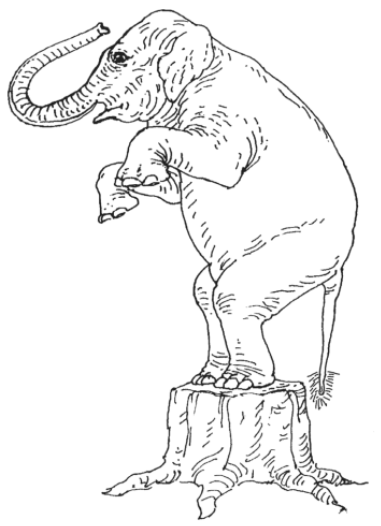
\includegraphics[height=4cm]{physics/figures/figure-unit-2-elephant.png}
% \end{center}

% \begin{center}
%     \begin{tikzpicture}
%         \node at (0,0) {\twemoji[width=3cm]{1f6cf}};
%         \draw[above=4.2mm,right=-6mm] (0,0) node {\twemoji[height=1.7cm]{elephant}};
%     \end{tikzpicture}
% \end{center}

% \begin{randomizechoices}[norandomize]
%     \choice The force of the Earth on the bed ($F_\text{bed-earth}$), and the force of the elephant on the Earth ($F_\text{earth-elephant}$).
%     \choice The force of the Earth on the bed ($F_\text{bed-earth}$), and the force of the elephant on the bed ($F_\text{bed-elephant}$).
%     \correctchoice The force of the Earth on the bed ($F_\text{bed-earth}$), and the force of the bed on the Earth ($F_\text{earth-bed}$).
%     \choice The force of the Earth on the elephant ($F_\text{elephant-earth}$), and the force of the bed on the elephant ($F_\text{elephant-bed}$).
% \end{randomizechoices}


\question
The graph below shows the velocity of a car that is moving in a straight line.

\begin{center}
    \begin{tikzpicture}
        \begin{axis}[width=7cm,
            height=5cm,
            xmin=0,xmax=50,
            ymin=0,ymax=35,
            xlabel={Time (s)},
            ylabel={Velocity (m/s)},
            xtick={0,10,...,50},
            ytick={0,10,...,30},
            axis lines=left,
            grid=both,
            clip=false,
            minor tick num=1,
            ]
            \coordinate (q) at (0,0);
            \fill (q) circle (2pt);
            \node[above] at (4.5,0) {$q$};
            \coordinate (r) at (10,10);
            \fill (r) circle (2pt);
            \node at (r) [above=2pt] {$r$};
            \coordinate (s) at (20,30);
            \fill (s) circle (2pt);
            \node at (s) [above=2pt] {$s$};
            \coordinate (t) at (30,30);
            \fill (t) circle (2pt);
            \node at (t) [above=2pt] {$t$};
            \coordinate (u) at (40,10);
            \fill (u) circle (2pt);
            \node at (u) [right=2pt] {$u$};
            \draw[thick] (q) -- (r) -- (s) -- (t) -- (u);
        \end{axis}
    \end{tikzpicture}
\end{center}

During which of the following intervals are forces on the car balanced?

\begin{randomizeoneparchoices}[norandomize]
    \choice $q$ to $r$
    \choice $r$ to $s$
    \correctchoice $s$ to $t$
    \choice $t$ to $u$
\end{randomizeoneparchoices}

\question 
A paper is sitting at rest on your desk.  Which of the following statements best describes this situation?

\begin{randomizechoices}[norandomize]
    \choice There are no forces acting on your paper.
    \choice Your paper has momentum and kinetic energy.
    \choice Your paper exerts no force on the desk since all the forces are balanced.
    \correctchoice There are forces acting on the paper, but they are all balanced.
\end{randomizechoices}

\question
A hockey player swings her hockey stick and strikes a puck.  Which of the following is the force pair to the stick pushing on the puck?

\begin{randomizechoices}[norandomize]
    \correctchoice The puck pushing on the stick.
    \choice The stick pushing on the player.
    \choice The player pushing on the stick.
    \choice The puck pushing on the player.
\end{randomizechoices}

\clearpage
\question 
Which of the following best describes the following person's motion?

% \begin{center}
%     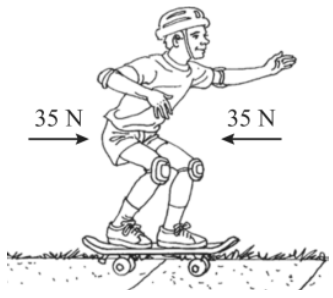
\includegraphics[width=6cm]{physics/figures/figure-unit-2-skater.png}
% \end{center}

\begin{center}
    \begin{tikzpicture}
        \draw (0,0) node {\reflectbox{\twemoji[height=2.5cm]{delivery truck}}};
        \draw[thick,<-,left=1.5cm] (0,0) -- (-4,0) node[above,pos=0.5] {400\,N};  
        \draw[thick,<-,right=1.5cm] (0,0) -- (+3,0) node[above,pos=0.5] {300\,N};  
    \end{tikzpicture}
\end{center}

\begin{randomizechoices}[norandomize]
    \correctchoice Moving and increasing their velocity, due to unbalanced forces.
    \choice Moving and decreasing their velocity, due to unbalanced forces.
    \choice Moving and increasing their velocity, up due to balanced forces.
    \choice Moving at a constant velocity, due to balanced forces.
\end{randomizechoices}

% \question 
% The picture below shows a student pulling in a rope that is attached to a wall.

% \begin{center}
%     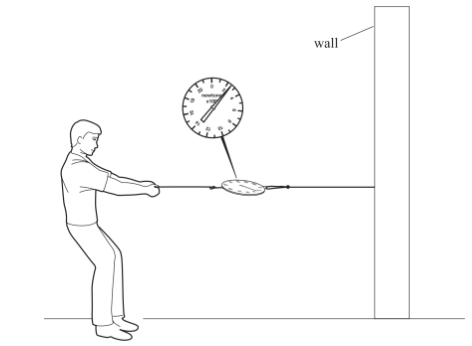
\includegraphics[width=6cm]{physics/figures/figure-unit-2-student.png}
% \end{center}

% Which statement correctly describes the amount of force applied by the wall on the student as they apply a \SI{250}{N} force?
    
% \begin{randomizechoices}[norandomize]
%     \choice The wall applies a force of 125 N against the student.
%     \correctchoice The wall applies a force of 250 N against the student.
%     \choice The wall applies twice as much force as the student.
%     \choice The wall applies no force since it is stationary.
% \end{randomizechoices}

\question 
When a bug hits the windshield of a car traveling at \SI{40}{mph}, the force of the bug on the windshield is

\begin{randomizechoices}[norandomize]
    \choice Greater than the force of the windshield on the bug.
    \choice Less than the force of the windshield on the bug.
    \correctchoice The same as the force of the windshield on the bug.
\end{randomizechoices}

\question
A student measuring the velocity and time of a toy car wrote down the following data.

\begin{center}
    \begin{tabular}{|c|c|c|c|c|c|c|}
        \hline
        \textbf{Velocity} (m/s) & \SI{4}{m/s} &  \SI{4}{m/s} & \SI{2}{m/s} & \SI{2}{m/s} & \SI{2}{m/s} & \SI{2}{m/s} \\ \hline
        \textbf{Time} (s) & \SI{0}{s} & \SI{2}{s} & \SI{4}{s} & \SI{6}{s} & \SI{8}{s} & \SI{10}{s} \\
        \hline
    \end{tabular}
\end{center}

What happened during the time interval between 2--4 seconds?

\begin{randomizechoices}[norandomize]
    \choice An unbalanced force was applied to the car increasing the car’s velocity.
    \correctchoice An unbalanced force was applied to the car, decreasing the car’s velocity.
    \choice A balanced force was applied to the car increasing the car’s velocity.
    \choice A balanced force was applied to the car, decreasing the car’s velocity.   
\end{randomizechoices}

% \question 
% Which of the following free body diagrams (FBDs) could represent the following image?

% \begin{center}
% \begin{tikzpicture}
%     \draw[fill=black!20] (0,0) rectangle ++(4,0.4);
%     \draw[fill=black!20] (0.5,0) rectangle ++(0.2,-2);
%     \draw[fill=black!20] (3.3,0) rectangle ++(0.2,-2);
%     \node[above=2.9mm] at (2,0) {\twemoji[height=1cm]{blue book}};
% \end{tikzpicture}
    
% \end{center}

% % \begin{center}
% %     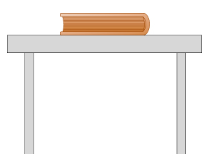
\includegraphics[width=6cm]{physics/figures/figure-unit-2-book.png}
% % \end{center}

% \begin{center}
%     \begin{tikzpicture}[scale=1.5]
%         \draw[thick,<->] (-1,0) -- (1,0);
%         \draw[thick,<->] (0,-1) -- (0,1);
%         \draw[fill=white] (-0.2,-0.2) rectangle ++(0.4,0.4) node[pos=0.5] {A};
%     \end{tikzpicture}
%     \hspace{2em}
%     \begin{tikzpicture}[scale=1.5]
%         \draw[thick,<->] (0,-1) -- (0,1);
%         \draw[fill=white] (-0.2,-0.2) rectangle ++(0.4,0.4) node[pos=0.5] {B};
%     \end{tikzpicture}
%     \hspace{4em}
%     \begin{tikzpicture}[scale=1.5]
%         \draw[thick,<->] (0,-1) -- (0,1.25);
%         \draw[fill=white] (-0.2,-0.2) rectangle ++(0.4,0.4) node[pos=0.5] {C};
%     \end{tikzpicture}
%     \hspace{2em}
%     \begin{tikzpicture}[scale=1.5]
%         \draw[thick,<->] (-1,0) -- (0,0);
%         \draw[thick,<->] (0,-1) -- (0,1);
%         \draw[fill=white] (-0.2,-0.2) rectangle ++(0.4,0.4) node[pos=0.5] {D};
%     \end{tikzpicture}
% \end{center}

% \begin{randomizeoneparchoices}[norandomize]
%     \choice Diagram A
%     \correctchoice Diagram B
%     \choice Diagram C
%     \choice Diagram D
% \end{randomizeoneparchoices}


% \question 
% Given the following image of a person on a bicycle, which of the following statements is correct about the cyclist’s motion?

% % \begin{center}
% %     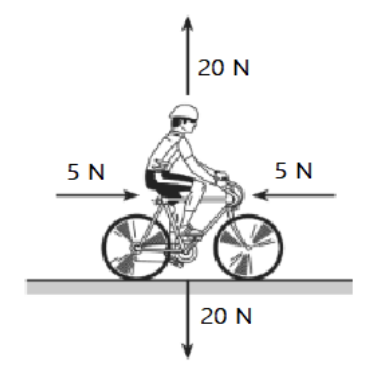
\includegraphics[width=6cm]{physics/figures/figure-unit-2-bicycle.png}
% % \end{center}

% \begin{center}
%     \begin{tikzpicture}
%         \node at (0,0) {\reflectbox{\twemoji[height=2cm]{man biking}}};
%         \draw[thick,<-,right=1.5cm] (0,0) -- (1,0) node[above,pos=0.5] {5\,N};
%         \draw[thick,<-,left=1.5cm] (0,0) -- (-1,0) node[above,pos=0.5] {5\,N};
%         \draw[thick,<-,above=1.2cm] (0,0) -- (0,2) node[right,pos=0.5] {20\,N};
%         \draw[thick,<-,below=1.2cm] (0,0) -- (0,-2) node[right,pos=0.5] {20\,N};
%     \end{tikzpicture}
% \end{center}

% \begin{randomizechoices}
%     \choice The person’s kinetic energy is changing with respect to time.
%     \choice The person’s velocity is changing with respect to time.
%     \correctchoice The person’s position is changing with respect to time.
%     \choice The person’s momentum is changing with respect to time.
% \end{randomizechoices}

\question 
Which of the following graphs represents an object with no kinetic energy?

\begin{center}
    \begin{tikzpicture}
        \draw[->] (0,0) -- (0,2.5) node[above,rotate=90,pos=0.5] {Velocity (m/s)};
        \draw[->] (0,0) -- (2.5,0) node[below,pos=0.5] {Time (s)};
        \draw[ultra thick] (0,1.5) -- ++(2,0);
        \node at (1.25,2.8) {\textbf{Graph A}};
    \end{tikzpicture}
    \hspace{2em}
    \begin{tikzpicture}
        \draw[->] (0,0) -- (0,2.5) node[above,rotate=90,pos=0.5] {Velocity (m/s)};
        \draw[->] (0,0) -- (2.5,0) node[below,pos=0.5] {Time (s)};
        \draw[ultra thick] (0,0) -- (2,2);
        \node at (1.25,2.8) {\textbf{Graph B}};
    \end{tikzpicture}
    \hspace{2em}
    \begin{tikzpicture}
        \draw[->] (0,0) -- (0,2.5) node[above,rotate=90,pos=0.5] {Position (m)};
        \draw[->] (0,0) -- (2.5,0) node[below,pos=0.5] {Time (s)};
        \draw[ultra thick] (0,1.5) -- ++(2,0);
        \node at (1.25,2.8) {\textbf{Graph C}};
    \end{tikzpicture}
    \hspace{2em}
    \begin{tikzpicture}
        \draw[->] (0,0) -- (0,2.5) node[above,rotate=90,pos=0.5] {Position (m)};
        \draw[->] (0,0) -- (2.5,0) node[below,pos=0.5] {Time (s)};
        \draw[ultra thick] (0,2) -- (2,0);
        \node at (1.25,2.8) {\textbf{Graph D}};
    \end{tikzpicture}
\end{center}

\begin{randomizeoneparchoices}[norandomize]
    \choice Graph A
    \choice Graph B
    \correctchoice Graph C
    \choice Graph D
\end{randomizeoneparchoices}

\clearpage

\printkeytable

% \question
% The following is a kinetic energy vs time graph made by a student doing a lab.  

% \begin{center}
%     \begin{tikzpicture}
%         \draw[->] (0,0) -- (0,3) node[above,pos=0.5,rotate=90] {Kinetic Energy};
%         \draw[->] (0,0) -- (3,0) node[below,pos=0.5] {Time};
%         \draw[ultra thick,domain=0:2.8] plot (\x,0.3*\x^2);
%     \end{tikzpicture}
% \end{center}

% Which of the following descriptions best represents what is happening to the object.

% \begin{randomizechoices}[norandomize]
%     \choice The forces are balanced and the kinetic energy is increasing.
%     \choice The forces are balanced and the kinetic energy is constant.
%     \choice he forces are unbalanced and the kinetic energy is constant.
%     \correctchoice The forces are unbalanced and the kinetic energy is changing.
% \end{randomizechoices}



\end{questions}
\end{document}

